\documentclass[12pt,a4paper]{article}

\usepackage[a4paper,margin=1in]{geometry}
\usepackage{graphicx}
\usepackage{booktabs}
\usepackage{amsmath,amssymb}
\usepackage{float}
\usepackage{hyperref}
\usepackage{xcolor}
\usepackage{listings}
\usepackage{enumitem}
\usepackage{fancyhdr}
\usepackage{longtable}
\usepackage{epstopdf}

\hypersetup{colorlinks=true,linkcolor=blue,urlcolor=blue}

\pagestyle{fancy}
\fancyhf{}
\lhead{ICS1512}
\rhead{Machine Learning Algorithms Laboratory}
\cfoot{\thepage}

\lstset{
language=Python,
basicstyle=\ttfamily\small,
numbers=left,
frame=single,
breaklines=true,
showstringspaces=false
}

\begin{document}

\begin{tabular}{|p{4cm}|p{11cm}|}
\hline
Experiment No. & 4 \\ \hline
Experiment Title & Support Vector Machine Application: Classification of Email Spam Data
\footnote{\textbf{GitHub Repository: }\url{https://github.com/Naren-Kandasamy/Machine_Learning_Lab-3122247001036}}\\ \hline
Student Name & Naren Kandasamy \\ \hline
Register Number & 3122247001036 \\ \hline
Faculty & Dr. Poreddy Ajay Kumar Reddy \\ \hline
Submission Date & 02/08/2026 \\ \hline
\end{tabular}

\vspace{0.5cm}
\noindent\textbf{Anaconda Activation Command:} \\
\texttt{source /opt/anaconda3/bin/activate anaconda-navigation}

\section{Objective}
This experiment set Logistic Regression against Support Vector Machines on the spam classification task, tried out a few different SVM kernels, and used RandomizedSearchCV to tune hyperparameters so the models would hold up reasonably well on unseen data rather than just fitting the training set well.

\section{Problem Statement}
With text-frequency features like these -- sparse, scaled, and fairly high-dimensional -- it's not obvious upfront whether a probability-based method or a margin-based one will draw the better boundary between spam and legitimate email. That's really the question this experiment is trying to answer: does Logistic Regression or SVM (and which kernel) come out ahead here.

\section{Dataset Description}
\begin{longtable}{|p{6cm}|p{8cm}|}
\hline
Dataset Name & Spambase Dataset \\ \hline
Dataset Source & Kaggle \\ \hline
Number of Samples & 4601 \\ \hline
Number of Features & 57 \\ \hline
Number of Classes & 2 (Spam, Ham) \\ \hline
Missing Values & None \\ \hline
Train-Test Split & 70\% Train, 30\% Test \\ \hline
\end{longtable}

\section{Exploratory Data Analysis}
An automated EDA function generated the usual 12-subplot summary of feature distributions and relationships, formatted per the lab spec (Times New Roman, 15pt, bold).

\section{Data Preprocessing}
The raw features here are frequency counts, and they don't all live on the same scale -- some word frequencies are tiny, others much larger. \texttt{StandardScaler} was used to bring everything to zero mean and unit variance before modeling. This matters more for SVM than it might seem at first: since the algorithm is built around Euclidean distance to find its margin, a feature with a naturally large range would otherwise end up dominating that calculation regardless of how useful it actually is. The train-test split (70:30) was stratified, so the spam/ham ratio stays roughly the same in both sets.

\section{Machine Learning Algorithm}
Two classifiers were built:
\begin{itemize}
    \item \textbf{Logistic Regression:} models the probability of the "spam" class directly through the logistic function. Simple, fast, and easy to interpret -- a good baseline to compare against.
    \item \textbf{Support Vector Machine (SVM):} tries to find the hyperplane that best separates the two classes with the widest possible margin. With kernels (Linear, Polynomial, RBF, Sigmoid) it can also handle cases where a straight line just won't do the job, by effectively working in a higher-dimensional version of the feature space.
\end{itemize}

\section{Experimental Setup}
\begin{tabular}{ll}
\toprule
Python Version & 3.10+ \\
Scikit-Learn Version & 1.0+ \\
IDE & VS Code \\
Operating System & Linux \\
Hardware & Standard CPU Workspace \\
\bottomrule
\end{tabular}

\section{Hyperparameter Selection}
\begin{tabular}{ll}
\toprule
Parameter & Value\\
\midrule
Logistic Regression Penalty & L2 \\
Logistic Regression C & 1000.0 \\
Logistic Regression Solver & liblinear \\
SVM Kernel & RBF \\
SVM C & 10.0 \\
\bottomrule
\end{tabular}

\section{Results}
\begin{tabular}{lc}
\toprule
Metric & Value\\
\midrule
Logistic Regression Accuracy & 0.9269 \\
Logistic Regression Precision & 0.9267 \\
Logistic Regression F1-score & 0.9267 \\
SVM (RBF Kernel) Accuracy & 0.9247 \\
SVM (RBF Kernel) Precision & 0.9246 \\
SVM (RBF Kernel) F1-score & 0.9244 \\
\bottomrule
\end{tabular}

\section{Result Visualization}

\begin{figure}[H]
\centering

\includegraphics[width=0.95\linewidth]{plots/eda_summary.eps}
\caption{Consolidated EDA summary showcasing the distributions of top predictive features within the Spambase dataset.}
\end{figure}
\textbf{Inference:}
Same pattern as before -- long tails in several of the character-frequency features, with most values sitting close to zero but a handful of outliers seemingly doing a lot of the work in telling spam apart from ham.

\begin{figure}[H]
\centering
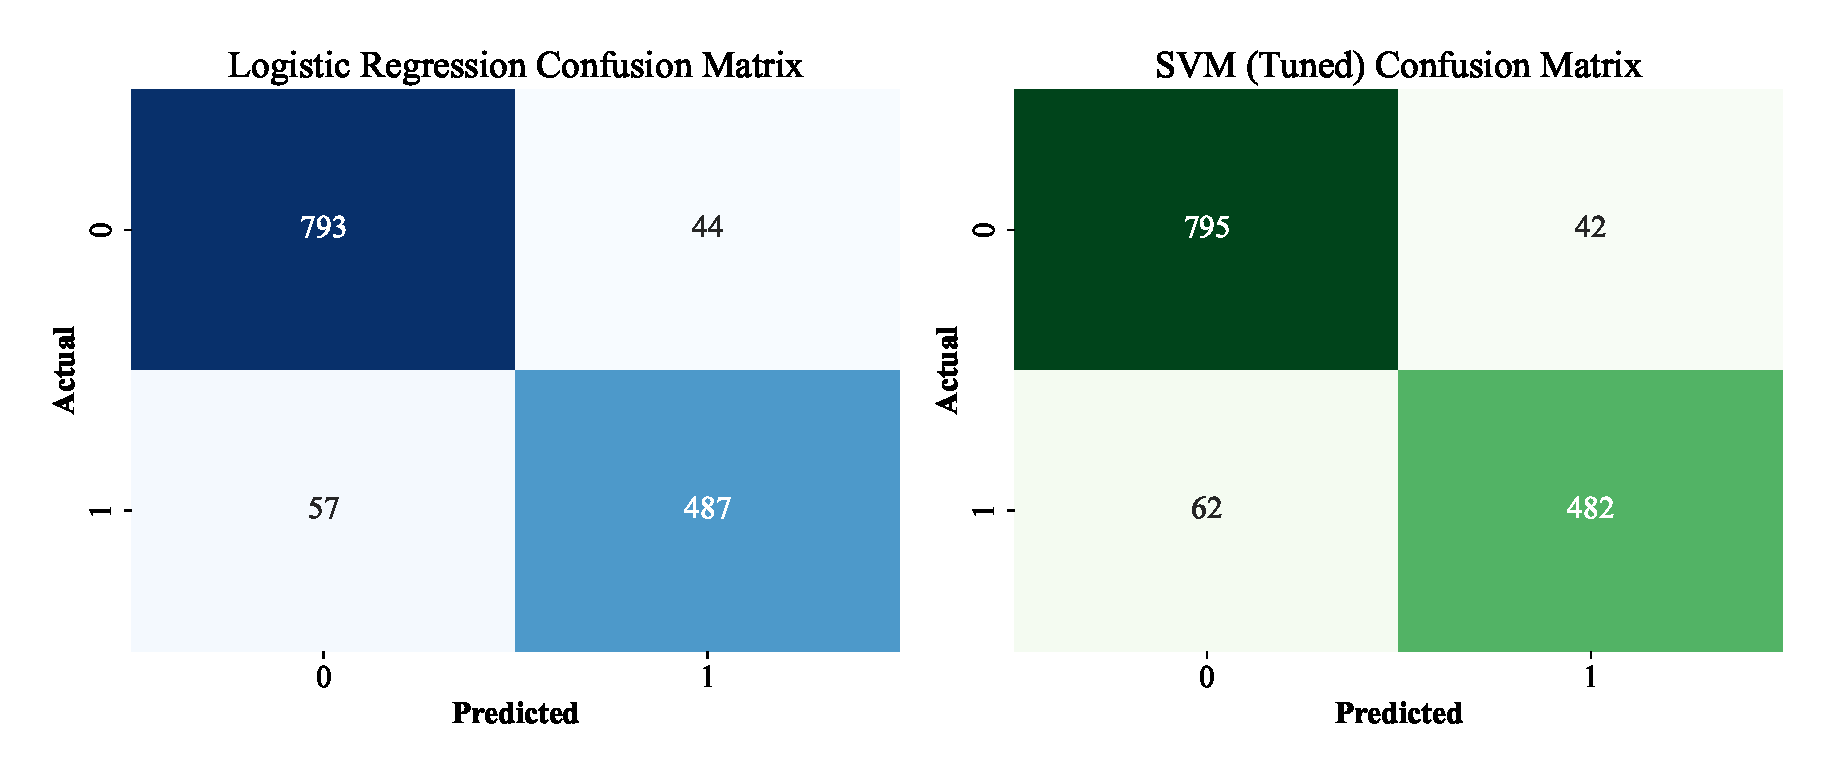
\includegraphics[width=0.9\linewidth]{plots/confusion_matrix.eps}
\caption{Confusion Matrix comparison between the tuned Logistic Regression and SVM models.}
\end{figure}
\textbf{Inference:}
Both confusion matrices look pretty clean, with strong diagonals. Logistic Regression has a very slight edge on this particular split, but honestly the two models are close enough that either would work fine in practice.

\begin{figure}[H]
\centering
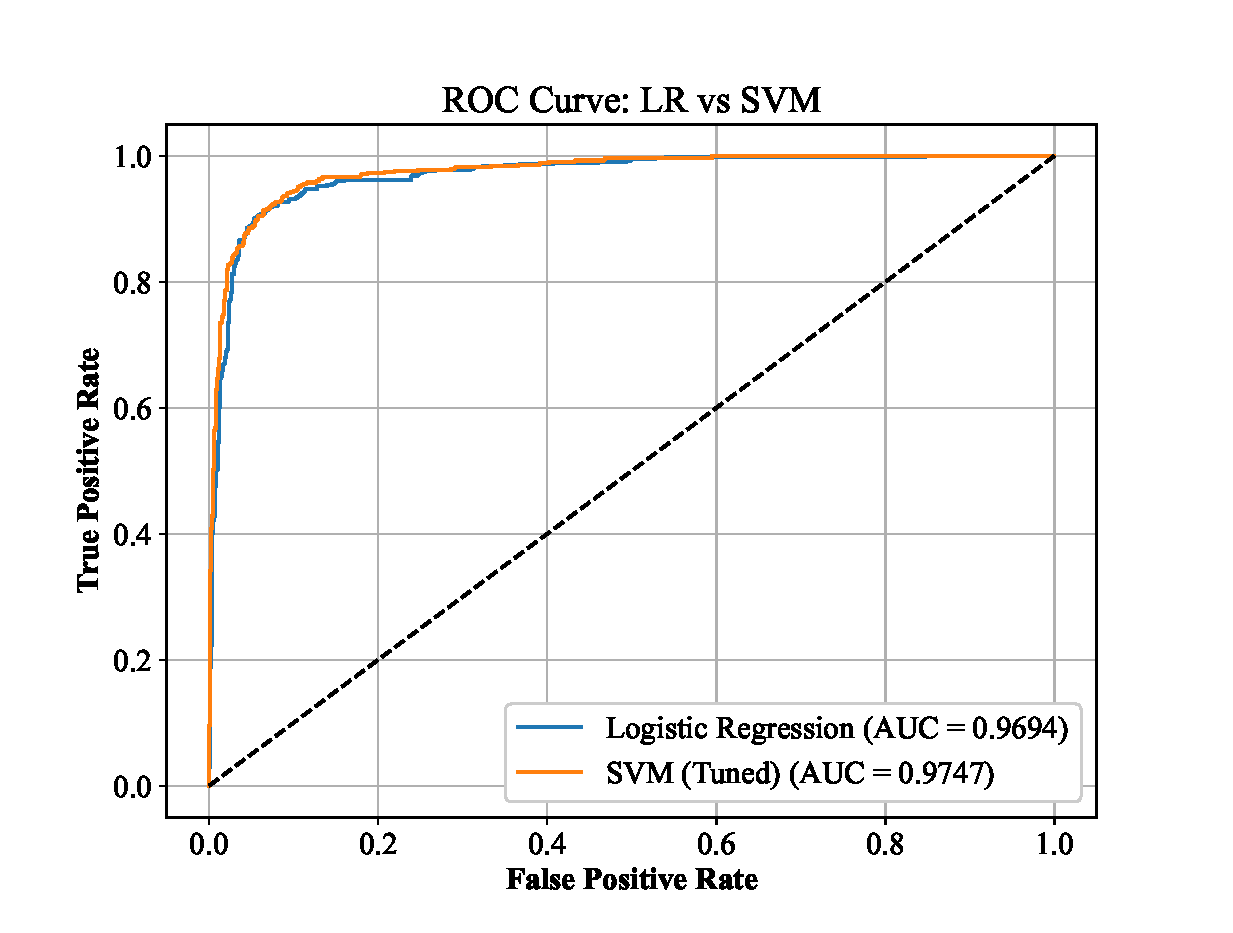
\includegraphics[width=0.6\linewidth]{plots/roc_curve.eps}
\caption{Receiver Operating Characteristic (ROC) curves demonstrating identical high AUC separation.}
\end{figure}
\textbf{Inference:}
The two ROC curves sit almost right on top of each other across the full range of thresholds, and both end up with a high AUC. There isn't much daylight between the two models here.

\section{Discussion}
The kernel comparison made it pretty clear early on that spam/ham data in this feature space is highly separable -- almost any reasonable model does well. After tuning, Logistic Regression and the RBF SVM ended up basically tied on the held-out test set, both around 92.5\% accuracy. Running 5-fold cross-validation gave a slightly more nuanced picture, though: the tuned SVM averaged 0.9331 accuracy across folds compared to 0.9272 for Logistic Regression, suggesting it generalizes just a bit more consistently even though the single test-split numbers looked nearly identical.

\section{Conclusion}
Both models turned out to be well suited to this kind of frequency-based text classification. If interpretability or training speed is the priority, Logistic Regression is the more practical choice, but the cross-validation results suggest the RBF-kernel SVM has a small edge in terms of raw generalization once it's properly tuned.

\section{References}
\begin{enumerate}
    \item Cortes, C., and Vapnik, V. "Support-vector networks." \textit{Machine Learning}, 1995.
    \item Hosmer Jr, D. W., Lemeshow, S., and Sturdivant, R. X. "Applied logistic regression." \textit{John Wiley \& Sons}, 2013.
\end{enumerate}

\end{document}
